\documentclass[../../main.tex]{subfiles}
\begin{document}

\begin{flushright}
  \footnotesize\textit{【自動文字起こし・要確認】}
\end{flushright}

{\bf [解答]}
$n$チームを$a_k$（$k=1,2,\ldots,n$）とおく．$n-2$勝$1$敗の$2$チームの選び方は${}_n\mathrm C_2=\dfrac{n(n-1)}{2}$通りである．以下，この$2$チームが$a_1,a_2$の時を考える．対称性から，$a_1$が$a_2$に勝つ時を考える．$\cdots①$

この時，考える対戦結果は次のようになる：$a_1$は$a_2$に勝ち，$a_3,\ldots,a_n$のうちある$1$チーム$a_k$（$3\le k\le n$）にのみ負ける．$a_2$は$a_1$に負け，$a_3,\ldots,a_n$には全て勝つ．
\begin{figure}[htb]
  \centering
  % n=5, k=4 の例．行のチームから列のチームを見た勝敗を記す．
  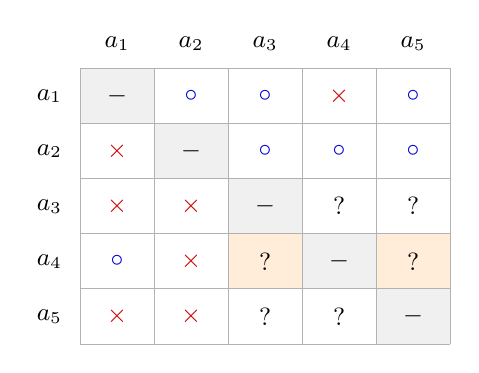
\begin{tikzpicture}[x=0.94cm, y=0.7cm, every node/.style={font=\small}]
    \fill[gray!12] (0,4) rectangle (1,5);
    \fill[gray!12] (1,3) rectangle (2,4);
    \fill[gray!12] (2,2) rectangle (3,3);
    \fill[gray!12] (3,1) rectangle (4,2);
    \fill[gray!12] (4,0) rectangle (5,1);
    \fill[orange!15] (2,1) rectangle (3,2);
    \fill[orange!15] (4,1) rectangle (5,2);
    \foreach \i in {0,...,5} {
      \draw[gray!60, thin] (0,\i) -- (5,\i);
      \draw[gray!60, thin] (\i,0) -- (\i,5);
    }
    \foreach \i/\name in {0/a_1,1/a_2,2/a_3,3/a_4,4/a_5} {
      \node[above=3pt] at (\i+0.5,5) {$\name$};
      \node[left=3pt] at (0,4.5-\i) {$\name$};
    }
    \node at (0.5,4.5) {$-$};
    \node[blue!85!black] at (1.5,4.5) {$\circ$};
    \node[blue!85!black] at (2.5,4.5) {$\circ$};
    \node[red!80!black] at (3.5,4.5) {$\times$};
    \node[blue!85!black] at (4.5,4.5) {$\circ$};
    \node[red!80!black] at (0.5,3.5) {$\times$};
    \node at (1.5,3.5) {$-$};
    \foreach \x in {2.5,3.5,4.5} \node[blue!85!black] at (\x,3.5) {$\circ$};
    \node[red!80!black] at (0.5,2.5) {$\times$};
    \node[red!80!black] at (1.5,2.5) {$\times$};
    \node at (2.5,2.5) {$-$};
    \node at (3.5,2.5) {$?$};
    \node at (4.5,2.5) {$?$};
    \node[blue!85!black] at (0.5,1.5) {$\circ$};
    \node[red!80!black] at (1.5,1.5) {$\times$};
    \node at (2.5,1.5) {$?$};
    \node at (3.5,1.5) {$-$};
    \node at (4.5,1.5) {$?$};
    \node[red!80!black] at (0.5,0.5) {$\times$};
    \node[red!80!black] at (1.5,0.5) {$\times$};
    \node at (2.5,0.5) {$?$};
    \node at (3.5,0.5) {$?$};
    \node at (4.5,0.5) {$-$};
  \end{tikzpicture}
  \caption{対戦結果の模式図（$n=5$, $k=4$；行の○は勝ち，×は負け，?は未確定）}
\end{figure}

この時，$a_1$は$a_k$にのみ負ける（$3\le k\le n$）．$a_2$は$a_3$〜$a_n$に全て勝つ．したがって，$a_3$〜$a_n$の中で，$a_k$以外は必ず$2$敗する．$a_k$が$2$敗以上する確率は$1-\left(\dfrac{1}{2}\right)^{n-3}$（$\because$排反）だから，のこる確率は
\begin{align}
  \left(\dfrac{1}{2}\right)^{2n-3}\left\{1-\left(\dfrac{1}{2}\right)^{n-3}\right\}
\end{align}

したがって，$a_1,a_2$が$(n-2)$勝$1$敗となる確率$P$は
\begin{align}
  P&=(n-2)\cdot2\left(\dfrac{1}{2}\right)^{2n-3}\left\{1-\left(\dfrac{1}{2}\right)^{n-3}\right\}\\
  &=(n-2)\left(\dfrac{1}{2}\right)^{2n-4}\left\{1-\left(\dfrac{1}{2}\right)^{n-3}\right\}
\end{align}

だから，全ての場合について足して，
\begin{align}
  n(n-1)(n-2)\left(\dfrac{1}{2}\right)^{2n-3}\left\{1-\left(\dfrac{1}{2}\right)^{n-3}\right\}．
\end{align}

\newpage

\end{document}
